%\lipsum[4-4]

Note: not in chronological order

\section{Architecture of proposed work}

\begin{figure}[h!]
	\centering
	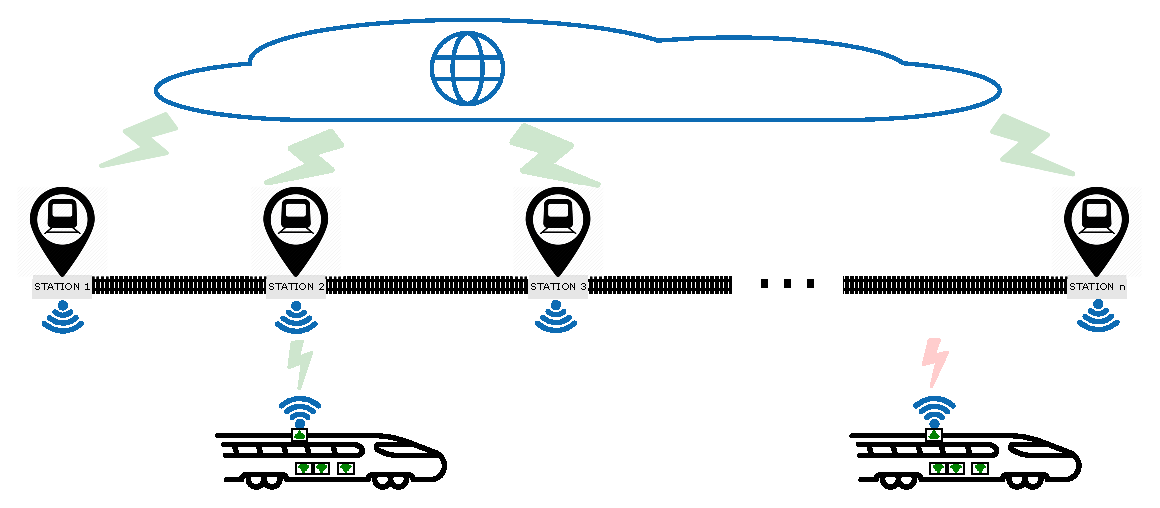
\includegraphics[width=1.0\textwidth,keepaspectratio]{figures/architecture}
	\caption{Architecture of proposed work.}
	\label{fig:architecture}
\end{figure}


\section{RTS wireless network}


\subsection{Purpose}
Model and simulate a WSN for energy measurement of RTS rolling stock, with an advanced network infrastructure (englobing both train WSN and station AP’s)

\subsection{Contribution}
%An energy measurement system in rolling stock does not require a broadband real-time/continuous communication (such as LTE), being possible to collect and store data in train data concentrator and, while the train is waiting at station for passenger exchange (which lasts for less than one minute), the data is transferred between train and station AP (and then to a remote server). Therefore, the contribution will be the cost reduction of information transmission of energy sensor network data

\begin{itemize}
	\setlength\itemsep{1em}
	\item An energy measurement system in rolling stock does not require a broadband real-time/continuous communication (such as LTE), being possible to collect and store data in train data concentrator and, while the train is waiting at station for passenger exchange (which lasts for less than one minute), the data is transferred between train and station AP (and then to a remote server).
	
	\item Therefore, the contribution will be the cost reduction of information transmission of energy sensor network data.
\end{itemize}

\subsection{Methodology}


\begin{itemize}
	\setlength\itemsep{0em}

	\item Modeling of energy sensor network of rolling stock: sensor nodes and data concentrator

	\item Modeling of infrastructure: train concentrators, station AP, station data “buffer” and station internet connection

	\item Implementation in simulation environment of such models, using NS3 simulator or similar

	\item Definition of “sensor data rate” as function of the line length-between-stations (?)
	
\end{itemize}





%%%%%%%%%%%%%%%%%%
%%%%%%%%%%%%%%%%%%
%%%%%%%%%%%%%%%%%%
\newpage
\section{Non-intrusive self-powered sensor node}

\subsection{Purpose}
In the scope of Shift2Rail, is expected to develop a smart meter for railways. The purpose is to model, simulate and implement a series of sensor nodes for current measurement in the transformer´s secondary windings. Assuming that the railway environment requires non-intrusive measurement devices and, if possible, self-powered, a set of requirements is then identified for the sensor node:

\begin{itemize}
	\setlength\itemsep{0em}
	\item Electrically non-intrusive (using hall-effect, rogowsky or current transformer principles; without the need for mechanically changing the windings)

	\item Self powered, if the current transformer has sufficient power capabilities

	\item With high processing capabilities, high acquisition frequency and sufficient amount of memory 

	\subitem Variable acquisition in tens of samples per second (according to the power quality standard of 15kHz <?>)

	\subitem Frequency analysis capability

	\subitem Capable of implement outlier detection algorithms 
\end{itemize}

\subsection{Contributions}

\begin{itemize}
	\setlength\itemsep{0em}
	\item New advanced sensor node for high current measurement

	\item Possible contribution: Given the measurement characteristics, a self powered wireless sensor node can implement features of high processing.
\end{itemize}
\subsection{Methodology}

4.	Methodology to be defined





%%%%%%%%%%%%%%%%%%
%%%%%%%%%%%%%%%%%%
%%%%%%%%%%%%%%%%%%
\newpage
\section{Rolling-stock traction transformer model}

\subsection{Purpose}
Model the train transformer with two perspectives:

\begin{itemize}
	\setlength\itemsep{0em}
	\item Efficiency estimation based on secondary measurements
	
	\item Evaluation of transformer operation towards fault detection
\end{itemize}


\subsection{Contributions}

\begin{itemize}
	\setlength\itemsep{0em}
	\item 	Possible contribution: an accurate model for train transformer, capable of efficient estimation of energy consumption based on secondary windings current measurements
	
	\item 	Possible contribution: assuming that the influence of transformer in the power life cycle cost is relevant (see note), the contribution will be the operation monitoring towards maintenance cost reduction.
\end{itemize}


\subsection{Methodology}

\begin{itemize}
	\setlength\itemsep{0em}
	\item Study failure rates of trains/transformers;
	
	\item Model in a simulation environment the power transformer

	\item Identify and model transformer failures

	\item Implement in sensor nodes an energy estimation mechanism based on the loss model of the transformer and sensor nodes measurements

	\item Implement in sensor nodes a frequency analysis towards operation monitoring

	\item Prepare and implement results in field operation
\end{itemize}
